%        File: siip.tex
%     Created: Mon Feb 27 08:00 AM 2017 C
% Last Change: Mon Feb 27 08:00 AM 2017 C
%
\documentclass[11pt]{article}

\usepackage[acronym,toc]{glossaries}
\include{acros}
\makeglossaries
\usepackage{fancyhdr}
\usepackage{pagecounting}
\usepackage[dvips]{color}
\usepackage{graphicx}
\usepackage{caption}
\usepackage{subcaption}
\usepackage{placeins}
\usepackage[hidelinks]{hyperref}
\usepackage{tabularx}

% Trying to bold my name in the bib
\usepackage{xstring}
\def\FormatName#1{%
          \IfSubStr{#1}{Huff}{\textbf{#1}}{#1}%
          }

          \usepackage[left=1in, right=1in, top=1in, bottom=1in]{geometry}
          \newcommand\bb[1]{\mbox{\em #1}}
          \def\baselinestretch{1.1}
          %\pagestyle{empty}
          \newcommand{\hsp}{\hspace*{\parindent}}
          \definecolor{gray}{rgb}{0.4,0.4,0.4}

          \newcommand{\authorname}{Kathryn~D.~Huff }
          \newcommand{\authoremail}{kdhuff@illinois.edu}
          \newcommand{\authorsite}{arfc.npre.illinois.edu}

          \begin{document}
          \title{Open Source, Collaborative Curriculum}
          \author{PI: Kathryn Huff\\Co-PI: Neal Davis}
          \maketitle

          \pagestyle{fancy}
          %\pagenumbering{gobble}
          %\fancyhead[location]{text}
          % Leave Left and Right Header empty.
          %\lhead{}
          %\rhead{}
          \lhead{\textcolor{gray}{PI: \authorname (NPRE)\\\authoremail}}
          \rhead{\textcolor{gray}{Collaborative Open Source Curriculum Development\\}}
          %\rhead{\textcolor{gray}{\thepage/\totalpages{}}}
          \renewcommand{\headrulewidth}{0pt}
          \renewcommand{\footrulewidth}{0pt}
          %\fancyfoot[C]{\footnotesize \textcolor{gray}{\authorsite}}

          \section{Problem}
          At this very moment, hundreds of professors in the United States are 
          simultaneously preparing lessons on transposing a matrix.
          They are doing so largely without receiving feedback from one another 
          or directly building on one another's experience 
          \cite{green_building_2014}. In this way, 
          professors spend an enormous amount of time duplicating curriculum 
          development efforts already tackled by colleagues. What's worse is 
          that these efforts are rarely, if ever, reviewed by, shared with, or 
          extended upon by peers.
          
          Open source software development provides an excellent 
          example of a possible solution.
          These communities have mastered distributed expert collaboration, 
          dynamic peer review, and de-duplication of effort. In open source 
          software, developers share code revisions in online repositories, 
          review one another's work in small chunks \cite{wilson_best_2014}, 
          and contribute back their own improvements to the main project.

          So, why aren't professors sharing their lesson materials online, 
          collaborating on canonical lesson sets, diffing and merging similar 
          lessons, and reviewing one another's learning materials? \textbf{Our 
          goal is to explore the possibility that curriculum development for 
          university courses can operate like open source software development 
          does.}
           
          Attempts at this have been made before. Most notable among 
          these is Software Carpentry (with which the PI and Co-PI are quite involved). 
          Software Carpentry teaches computational skills for scientists using 
          a shared curriculum hosted on GitHub. Unfortunately, our experience showed that 
          forks of the original material tend to diverge without any strong 
          incentive for contribution back to the master material 
          \cite{wilson_software_2014,wilson_software_2014-1}. We expect that fine-grained modularity 
          of lesson components and a clear dependency graph of prerequisite 
          modules for each lesson may assist in overcoming the challenges 
          encountered by Software Carpentry and others.

          \section{Proposed Solution}
          We propose a small-scale proof-of-concept for collaborative, open 
          source, curriculum development to improve the transfer of lessons 
          learned between instructors of the same course (either at a single 
          university or among different campuses). This prototype collaboration 
          will provide a template which could be adopted for collaboration 
          among faculty teaching courses with an inherently larger scale (e.g. 
          CS101)

          Faculty in Nuclear Engineering from four institutions\footnote{Paul 
          Wilson at (UW Madison), Steven Skutnik (UT Knoxville), Jeremy Roberts 
          (Kansas State University), Anthony Scopatz (University of South 
          Carolina), and Robert Borrelli (University of Idaho)} have agreed to be participants in 
          this prototyping effort. We all currently use 
          \href{https://github.com}{GitHub} to store, 
          revise, and collaborate on research, especially source code. 
          Additionally, this select group already started to host our course 
          curricula online as well, but these are typically single author 
          repositories (e.g. \cite{huff_npre412_2017}).

          The participants will collaborate on a master set of learning 
          modules for an upper-division course in nuclear engineering : 
          The Nuclear Fuel Cycle. In the near term, we will develop fine 
          grained lessons which may be mixed and matched to meet the 
          learning objectives. The curriculum will be hosted on GitHub, 
          tested by all of us, and improved continually.

          \subsection{Open Source Workflow}
          Development of this proof-of-concept curriculum will be undertaken 
          similarly to an open source software project. 
          In particular, this work will emulate features of open source software development 
          that cultivate distributed collaboration. In open source, for 
          example, new code features are described in \emph{issues} or 
          \emph{tickets} and discussed before implementation. Small, atomic 
          changes are reviewed before they are merged into the 
          \emph{repository}. These discussions and incremental reviews nurture 
          communities of practice.

          In a typical open source project, a main copy of the 
          repository (or main \emph{fork}) holds the 
          official copy of the software package. Individual developers each have their own 
          \emph{forks} where they can work on features and 
          bug fixes. When the developer makes changes that are ready for prime 
          time, they make a ``pull request'' to the main \emph{fork}. That 
          \emph{pull request} is 
          reviewed by their collaborators, and it is eventually merged into the 
          main \emph{fork} where it can be used by all. Figures 
          \ref{fig:sub1} and \ref{fig:sub2} show how this open source software 
          development workflow
          can be leveraged toward course development.

          \begin{figure}
                  \centering
                  \begin{subfigure}{.4\textwidth}
                            \centering
                              \includegraphics[width=.8\linewidth]{git-flow}
        \caption{This figure, from \cite{scopatz_effective_2015}, captures a 
                          process, often called Git Flow, through which a new 
                          feature or bug fix enters a piece of open source 
                          software.}
                                  \label{fig:sub1}
                  \end{subfigure}\hfill%
                  \begin{subfigure}{.4\textwidth}
                            \centering
                              \includegraphics[width=.8\linewidth]{siip-flow}
  \caption{This adaptation imagines the process in the context of learning module development, using the same git version control system and GitHub repository hosting framework.}
                                  \label{fig:sub2}
                  \end{subfigure}
                  \label{fig:test}
          \end{figure}
          \FloatBarrier

\iffalse
          Doing code review at the end of the work isn't useful. What works is 
          incremental code review. This proposal suspects that the same is true 
          for curriculum review.  \cite{wilson_software_2014}.

          Education is an inherently distributed system, but this need not be a hinderance to collaboration.

          Scientists are more than happy to build upon one another's work, form 
          collaborations with others in their field. But, 
          when it comes to educating, where is the sharing of lessons learned 
          and collaboration? 
\fi

          \subsection{Kick-Off Workshop}
          A two-day kick-off workshop (\$15K) at UIUC will allow the 
          participants to sketch the initial framework of 
          the collaboration and coordinate logistics. The workshop will 
          deliver:

          \begin{itemize} 
                  \item learning objectives\cite{bloom_bloom_1984} for the 
                          course
                  \item a concept map\cite{novak_concept_1990} for the course
                  \item a list of fine-grained lesson topics
                  \item a directed acyclic graph describing dependencies among 
                          lessons
                  \item individual assignments for curriculum development
                  \item decisions to adopt specific raw formats for lesson content
                        (markdown vs. \LaTeX, Jupyter vs MATLAB, etc.)
                  \item a repository structure for organizing the lesson 
                          material (at this stage, compatibility with 
                          frameworks like RELATE 
                          \cite{kloeckner_relate_2017,kloeckner_relate_2017} 
                          and tools like PrarieLearn 
                          \cite{west_prairielearn:_2015} will be considered)
          \end{itemize} 

          Invited participants in the first workshop will include:
          \begin{itemize}
                  \item UIUC PI Huff and UIUC Co-PI Davis
                  \item external collaborating Professors Wilson, Roberts, 
                          Borrelli, Skutnik, and Scopatz
                  \item up to 5 UIUC professors who may be likely to extend 
                          this work in the future for their own courses.
          \end{itemize}

          \subsection{Interim Period}
          Between Workshops, work will commence on developing 
          lessons. These lessons will be submitted by pull request to the main 
          repository and each lesson will include:
          \begin{itemize} 
                  \item associated learning objectives (identified previously)
                \item content (e.g. speaking notes, presentation material, 
                        derivations, worked examples, active learning  
                          exercises, external readings, videos, images)
                  \item learning assessments (e.g. project descriptions, exam questions) 
          \end{itemize} 

          Interactions will commence primarily via issues, pull requests, and 
          reviews on GitHub during this time. Meanwhile, monthly video 
          conferences will help to spur high-level conversation onward.
          Co-PI Davis will be invited to engage in these video conference as 
          part of action research toward the final 
          As progress is made, lessons learned will be recorded by all 
          participants in a draft instruction manual. 

          \subsection{Retrospective Workshop}
          A two-day retrospective workshop (\$15K) at UIUC will wrap up the 
          project. Discussion concerning the process will allow reflection as 
          well as a collection of lessons learned.
          Experiences live testing the developed course material (for example 
          in NPRE412 at UIUC in Fall 2017) will be shared and suggested 
          improvements will be captured as feature requests on GitHub.  
          The lessons learned from the year-long process will be captured:
          
          \begin{itemize}
                  \item in a template repository 
                  \item and in a collaboration instruction manual 
          \end{itemize}

          These products will be produced for use by other groups of faculty 
          seeking to collaborate in a similar way.

          Invited participants in the retrospective workshop will include:

          \begin{itemize}
                  \item UIUC PI Huff and UIUC Co-PI Davis
                  \item external collaborating Professors Wilson, Roberts, 
                          Skutnik, and Scopatz
                  \item up to 20 UIUC professors interested in extending this 
                          work in the future for their own courses.
          \end{itemize}


          \section{Potential Impact}
          This work will have immediate student and faculty outcomes at UIUC, 
          USC, KSU, UT Knoxville, and UW Madison. It will additionally have long term 
          student and faculty outcomes at UIUC. Beyond this, it may have 
          institutional outcomes at UIUC. 
          
          This work will provide an important proof of concept for groups of 
          instructors willing to collaborate on open source curriculum for:
          \begin{itemize}
                  \item core courses with many sections in a single university
                  \item niche courses taught by a select group of professors across 
          universities
                  \item fundamental courses in small fields (e.g. nuclear engineering)
          \end{itemize}

          \paragraph{Student Outcomes}
          Students enrolled in NPRE412 at UIUC and peer courses at partner 
          institutions (USC, UT-Knoxville, Kansas State University, and 
          UW-Madison) will have an improved experience. Their 
          curriculum will be bolstered by the comprehensive concept maps 
          underlying their coursework\cite{concept_maps}, as well as exercises 
          and assessment tools reviewed and improved by expert professors at 
          peer institutions. 

          \paragraph{UIUC Faculty Outcomes}
          The effort of developing curriculum in this way may be labor 
          intensive initially. However, if the experience is similar to that of 
          open source software, the maintenance effort will reduce 
          substantially. Minor improvements and updates to the curriculum 
          contributed by colleagues will be effectively 'free' in the long 
          term. 

          \paragraph{UIUC Institutional Outcomes}

          Fame, glory.

          \paragraph{External Outcomes}

          Of perhaps most relevance in the context of this work is the 
          potential impact externally. This effort should spawn an 
          instruction-centric community of 
          practice among colleagues previously primarily connected by research 
          in their specific technical subdomain. 

          \section{Timeline and Deliverables}
          \subsection{Timeline}
          The timeline will be bookended by two workshops, a kickoff workshop 
          and a retrospective workshop. In the intervening time, consistent 
          communication through GitHub's collaboration framework, a Slack 
          channel, an email listhost, a shared Google Drive folder, and  

          \begin{itemize}
                  \item[July 2017] 1st Workshop
                  \item[.] 
                  \item[.] 
                  \item[.] 
                  \item[July 2018] Retrospective Workshop
          \end{itemize}

          \subsection{Deliverables}

          \subsubsection{Learning Objectives List}
          \subsubsection{Concept Map}
          \subsubsection{Learning Dependency Graph}
\begin{figure}[htb!]
        \begin{center}
                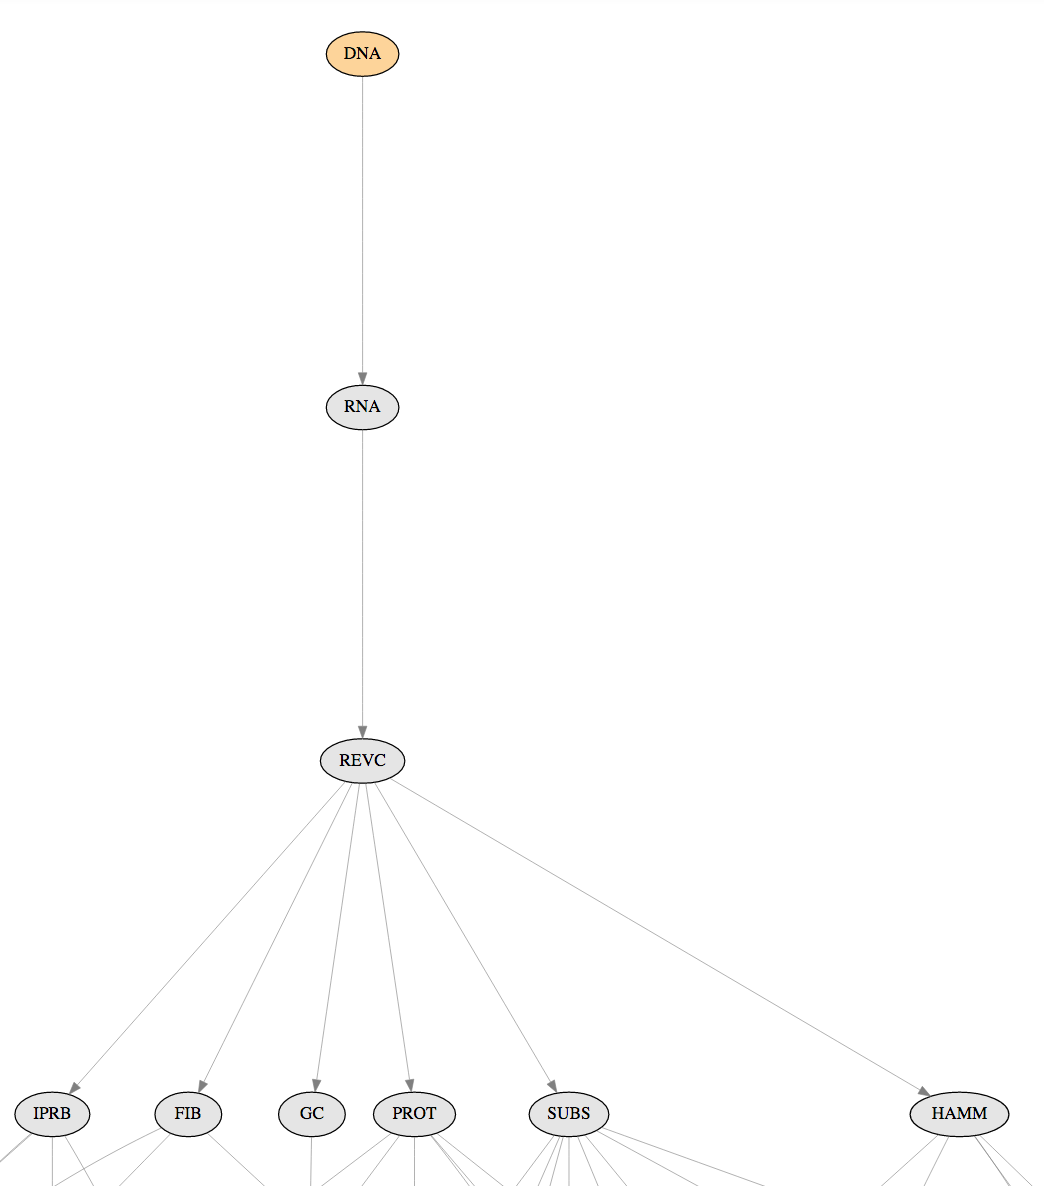
\includegraphics[height=0.5\textheight]{rosalind.png}
        \end{center}
        \caption{Rosalind.info has a graph of exercises and their dependencies.}
        \label{fig:rosalind}
\end{figure}
          \subsubsection{Lesson Materials}


          \section{Budget}
          The two workshops will be hosted at the Illini Union, where a meeting 
          room will be reserved. Visiting 
          invited workshop participants will be flown to Urbana-Champaign and 
          lodged at the Illini Union Hotel.

\begin{table}[htb]
        \begin{tabularx}{\textwidth}{| X |c|c|c|c|c|}
        \hline
        \textbf{Event} & \textbf{Item} & \textbf{Cost} & \textbf{Units} & \textbf{\$} & \textbf{Notes}\\ 
        \hline
Kick-off Workshop&Meeting Room&744&2&1488&Allerton, all day package\\
&Lodging&150&24&3600&Allerton guest rooms\\
&Flights&800&6&4800&Estimated\\
&Taxi&20&12&240&\\
&Incidentals&100&6&600&\\
&Continental breakfast&8.5&24&204&Working breakfasts, Allerton\\
&Dinner&30&24&720&In Champaign-Urbana\\
\hline
Retrospective Workshop&Meeting Room&50&2&100&Illini Union\\
&Projector&300&4&1200&Illini Union\\
&Lodging&150&24&3600&Illini Union Hotel\\
&Flights&800&6&4800&Estimated\\
&Taxi&20&12&240&\\
&Incidentals&100&6&600&\\
&Continental breakfast&8.5&24&204&University Catering\\
&Coffee Service&32.5&4&130&\\
&Lunch&15&24&360&University Catering\\
&Dinner&30&24&720&In Champaign-Urbana\\
        \hline
        &\textbf{Total}&&&\textbf{23606}&\\
        \hline
\end{tabularx}
\end{table}

          \section{Departmental Support}
          The Department of Nuclear, Plasma, and Radiological Engineering will 
          support this work in kind with release time for Kathryn Huff through 
          her Start-Up funds.  Additionally, NPRE will support workshop activities 
          with administrative effort and by providing space. Finally, 
          collaborating external participants will contribute in kind with 
          summer time hours.


          \bibliographystyle{katyunsrt}
          \bibliography{2017-siip}


          \end{document}


